\section{Introduction}
We present here a framework for passing messages between discrete points on a finite lattice, where each point updates its internal data (and thus the messages it sends) based on messages received.  Each point is uniquely connected to other points and so has its own \emph{neighbourhood}, being the specific other points it communicates with.  A key aspect of this \emph{\gls{nmp}} computation is that the messages to a given neighbour depend upon the messages received previously from \emph{all} neighbours, \emph{except} the neighbour to which the current message is sent.    This necessarily means that in \gls{nmp} each grid location must have at least two neighbours.  A single neighbour cannot form a meaningful neighbourhood.  We focus on the \emph{square lattice} but emphasise that \gls{nmp} applies equally to lattices of any shape or dimension.

In this paper, we term the individual computational units in the lattice \emph{\glspl{pe}}.\footnote{We derive the short form ``\gls{pe}'' from ``processing element'' in the same way that ``pixel'' is derived from ``picture element''.}  These are the logical base units for computation for our purposes and are represented by \gls{cps} top-level cells.  A visual example of the \gls{nmp} process for the \emph{\gls{fne}} on the square lattice is shown in \cref{fig:nmp:gridmessaging}.\footnote{The \(\Sigma\) and \(\Pi\) in the centre circle relate to Sum-Product Belief Propagation and its approach for computing new messages and can be ignored in this paper.  They will be relevant in Part Two.}  A \gls{pe} in the grid received messages from its neighbours to the left, right, and bottom at generation \(t - 1\), and has used the data from those messages in preparing its new message to be sent to the neighbour above at iteration \(t\).  The same is performed for each other neighbour too.

\begin{figure}
    \centering
    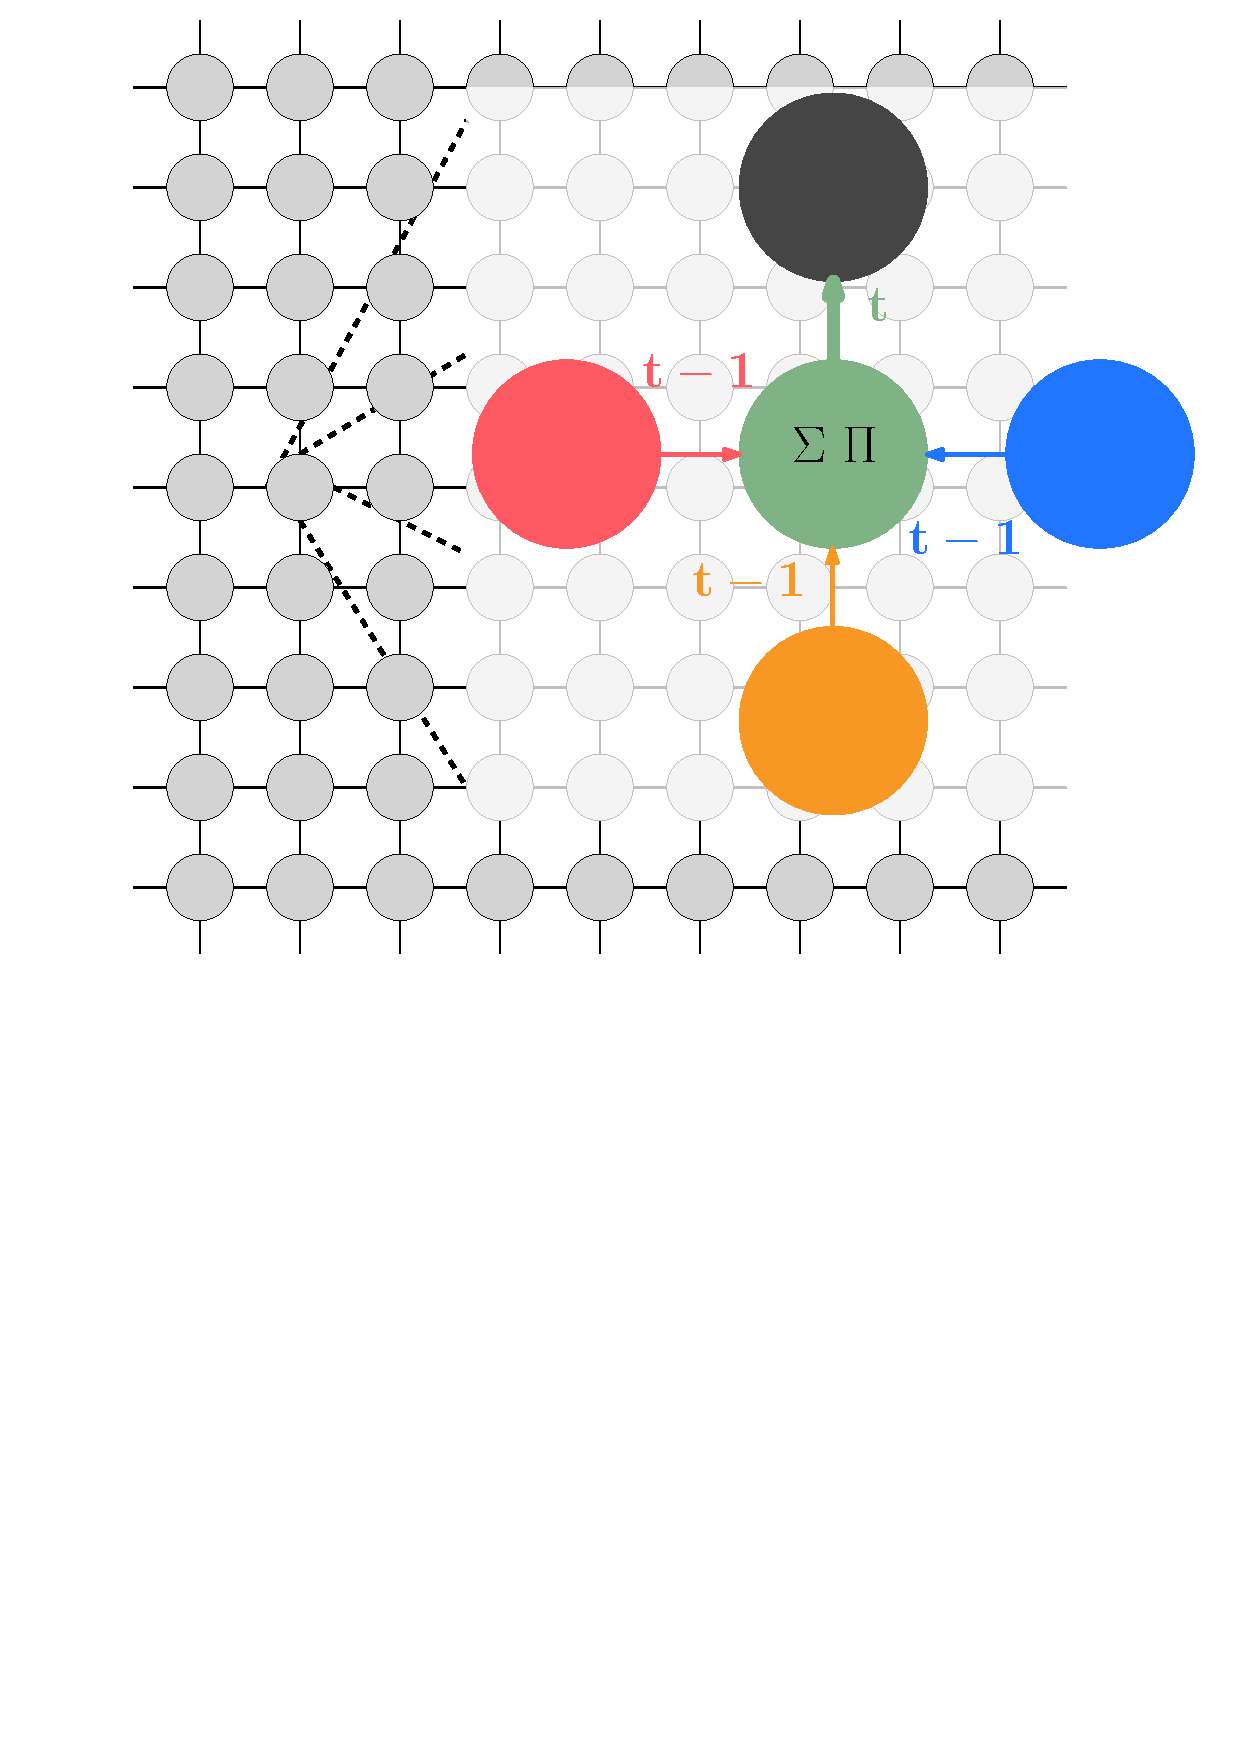
\includegraphics[keepaspectratio,width=1.0\linewidth]{chapters/nmp/images/bp_diagram_recoloured.pdf}
    \caption[Diagram of the central concept of \gls{fne} \acrlong{nmp} on a grid]{Diagram of the central concept of \gls{fne} \gls{nmp} on a grid \cite{lbpmpsmpic}.  Each circle represents a \gls{pe}.  The central \gls{pe} needs to compute a new message to send at time \(t\) to the \gls{pe} above it, so it performs a computation to combine the results of the messages received from the other three neighbouring cells at time \(t - 1\) (indicated by the thin and fat arrows).  The same is applied to every other neighbour, too.}
    \label{fig:nmp:gridmessaging}
\end{figure}

Conceptually, there are two distinct aspects of the \gls{nmp} process.  The message passing itself, which occurs externally to \glspl{pe} over channels connected to other \glspl{pe}, and the data/message updates, which occur internally.  The focus of this paper is the external side, and we use communication with an oracle to represent the internal computation, which is largely orthogonal to the inter-\gls{pe} communication.

There are (at least) two separate ways to model the \glspl{pe}' communication:  a \emph{\gls{gs}} system-wide view, where the states and steps taken occur across the system as a whole and every \gls{pe} carries out its operations simultaneously according to the same rules.  Or, a per-\gls{pe} view, where each \gls{pe} has its own state and advances \emph{asynchronously} without regard to others' objects, states, and rulesets.  We explore both and find in the process that an intermediate third, \emph{\gls{ls}}, model arises naturally as a hybrid of the other two.

The modelling and implementation of \gls{nmp} proves unexpectedly challenging.  On the surface, it seems as if it should be a straightforward problem, and in the synchronous form (\cref{sec:nmp:systemwide}) it \emph{is} reasonably simple.  It requires only nine rules, most of which have exactly one term on both the left-hand- and right-hand-sides and none of which use promoters or inhibitors (see \cref{sec:lr:cpsystems} for more on these concepts).

The challenge arises in modelling the asynchronous version.  The possibility of messages for the same iteration arriving at separate times necessitates bookkeeping.  There is a need to track from which neighbours messages have been received for a given generation to decide which neighbours the \gls{pe} is now ready to send a new message to.  This gives rise to inescapable complexity and opens up the undesirable possibility of deadlock through an unsuitable design.

This paper makes two main contributions:  Firstly, it is the first to use an antiport rule in \gls{cps}.  Secondly, to the best of our knowledge, it is also the first time asynchronous \gls{nmp} has been explored in \emph{any} context, P~systems or otherwise.  The paper begins with a summary of \gls{cps}, before describing a straightforward synchronous \gls{nmp} system using the aforementioned antiport rule.  Then, it provides an asynchronous \gls{pe}-specific version of the same followed by an adaptation of the asynchronous system to a \gls{ls} system. Next is a short example of a potential evolution of the asynchronous system to clarify the expected operation of the system.  Lastly, this paper analyses the asynchronous system and performs comparative computer experiments for all three systems before concluding.  The analysis proves that the asynchronous system sends precisely the same number of messages as the synchronous system (one per generation per neighbour) but that the data used to compute new messages may vary slightly depending on the ordering of messages received.  Furthermore, the empirical results verify the operation of the asynchronous system and support our hypothesis that the \gls{ls} and asynchronous systems are faster than an equivalent \gls{gs} version.